\section{Gilda dei protettori della Sila Devoti a San Francesco e ai
Lupi}\label{gilda-dei-protettori-della-sila-devoti-a-san-francesco-e-ai-lupi}

Tags: Organizzazione Creatore: Davide, Lorenzo

\section{\texorpdfstring{\textbf{Gilda dei Protettori della Sila Devoti
a San Francesco e ai
Lupi}}{Gilda dei Protettori della Sila Devoti a San Francesco e ai Lupi}}\label{gilda-dei-protettori-della-sila-devoti-a-san-francesco-e-ai-lupi-1}

\begin{center}\rule{0.5\linewidth}{0.5pt}\end{center}

\begin{center}\rule{0.5\linewidth}{0.5pt}\end{center}

\begin{figure}
\centering

\includegraphics{a-golden-coin-with-a-face-of-a-wolf-engraved-in-it-.png}
\caption{a-golden-coin-with-a-face-of-a-wolf-engraved-in-it-.png}
\end{figure}

Informazioni Generali

Tipo: Gilda

Struttura:

Regione: Valtara

Fondatore: Paladini di San Francesco

Membri: I Protettori

Alleati: Ordine dei Paladini di San Francesco

Nemesi:

\subsection{1. Descrizione Generale}\label{descrizione-generale}

\begin{center}\rule{0.5\linewidth}{0.5pt}\end{center}

\begin{figure}
\centering
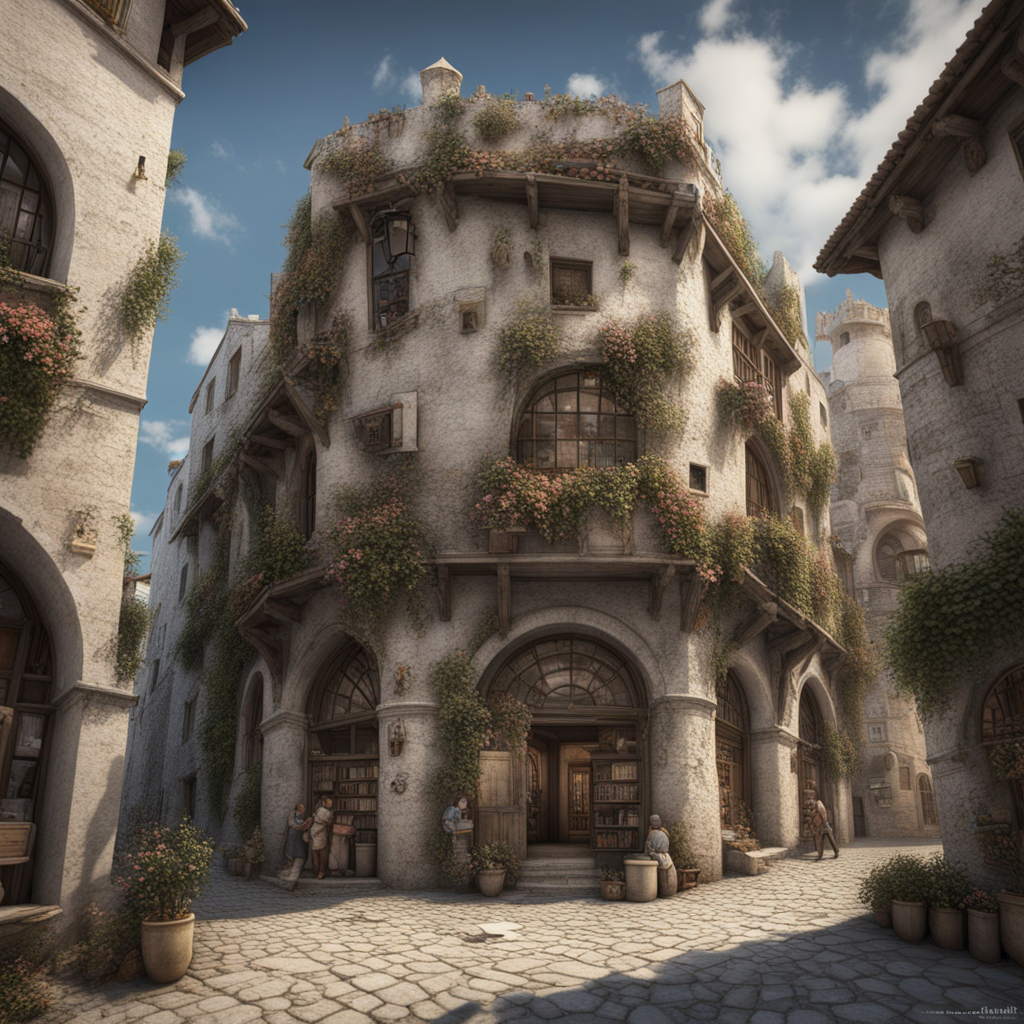
\includegraphics{generate-an-image-depicting-the-exterior-of-il-pane-quotidiano-newspaper-headquarters-in-the-medie.png}
\caption{generate-an-image-depicting-the-exterior-of-il-pane-quotidiano-newspaper-headquarters-in-the-medie.png}
\end{figure}

La Gilda dei Protettori della Sila Fedele a San Francesco e ai Lupi,
nota semplicemente come Gilda dei Protettori, è un organizzazione
fondata dai paladini e composta da avventurieri devoti a San Francesco e
ai valori della giustizia e dell'onore. Con base a Kos, la città natale
di San Francesco, operano in difesa del bene e della compassione.
Accettano membri diversificati, impegnandosi in missioni di
pacificazione e lotta al male in tutta Valtara. Collaborano strettamente
con le autorità locali per mantenere l'ordine e la sicurezza.

\emph{Il Pane Quotidiano} è un rinomato giornale nel mondo di Valtara,
noto per la sua dedizione nell'offrire una copertura completa e accurata
degli avvenimenti in . Fondata con l'obiettivo di soddisfare la sete di
conoscenza e la curiosità dei suoi lettori, questa organizzazione
giornalistica ha stabilito la sua sede principale nella maestosa città
di Kos.

\begin{quote}
``Giuro fedeltà ai compagni e alla gilda. Giuro fedeltà al lupo che con
la sua forza guida i nostri passi. Giuro fedeltà allo spirito di San
Francesco che ci protegge in ogni viaggio. Lupi alé! Lupi alé! Lupi
alé!''

-Giuramento della gilda
\end{quote}

\subsection{2. Storia}\label{storia}

\begin{center}\rule{0.5\linewidth}{0.5pt}\end{center}

La Guerra del Sangue fu un evento tragico che rimase impresso nella
memoria dei paladini dell'
\href{Ordine\%20dei\%20Paladini\%20di\%20San\%20Francesco\%20e8fd423783714ddeb11ec757edea519b.md}{Ordine
dei Paladini di San Francesco} come un duro ammonimento della perfidia
umana e della necessità di rimanere sempre vigili contro le forze oscure
che cercano di distruggere il bene.

Per questo motivo decisero di riorganizzare la milizia costituita in
occasione della guerra, fondando una gilda, la Gilda dei Protettori
della Sila Devoti a San Francesco e ai Lupi, nota in seguito come la
Gilda dei Protettori. La gilda sarebbe stata aperta a chiunque fosse
desideroso di combattere il male, purché avesse una forte fede in San
Francesco e nei valori della giustizia e della compassione. La Gilda dei
Protettori della Sila Devoti a San Francesco e ai Lupi divenne
rapidamente un'organizzazione rispettata e temuta in egual misura.

Non solo la Gilda ripristinò la reputazione dell'ordine dei Paladini di
San Francesco, ma la superò, diventando una forza potente e influente
nella lotta contro il male. La loro determinazione e la loro dedizione
alla causa ispirarono molti altri, portando la Gilda oltre i confini
della città natale. Oggi, dopo più di 20 anni dalla sua nascita, la
Gilda è diventata un'organizzazione complessa e ramificata, con una sede
in ogni grande città di Valtara. Nonostante sua nobile origine, la Gilda
permette ai suoi membri di accettare i più disparati incarichi, a volte
al limite dell'etica. Questo elemento è preso ad esempio dai critici più
feroci dell'organizzazione, che credono che la Gilda abbia poco a che
fare con l'antico Ordine dei Paladini di San Francesco, poiché ormai
composta da mercenari al soldo del miglior offerente.

\subsection{3. Valori}\label{valori}

\begin{center}\rule{0.5\linewidth}{0.5pt}\end{center}

I valori chiave della Gilda dei Protettori includono la giustizia, la
compassione, la fedeltà, il coraggio, l'unità, il sacrificio, la fede,
l'onestà, la determinazione e la responsabilità. Questi principi guidano
i membri della Gilda nelle loro azioni e decisioni mentre lottano per
proteggere gli innocenti, preservare la giustizia e combattere il male
in modo equo e determinato. La Gilda promuove l'unità e la cooperazione
tra i suoi membri, insieme alla compassione verso coloro che sono in
difficoltà. La fede in San Francesco è un pilastro importante, e
l'onestà e l'integrità sono altamente valorizzate. I Protettori sono
noti per il loro coraggio e la loro determinazione nell'affrontare le
sfide, e sono pronti a fare sacrifici personali per il bene comune.
Infine, la responsabilità verso la protezione degli innocenti e il
perseguimento della giustizia è un obiettivo centrale per la Gilda.

\subsection{4. Cultura}\label{cultura}

\begin{center}\rule{0.5\linewidth}{0.5pt}\end{center}

La cultura della Gilda dei Protettori è profondamente radicata nei
valori di devozione a San Francesco e nella sua connessione con la città
di Kos, luogo di nascita del San. Questo legame con San Francesco
rappresenta il cuore e l'anima della Gilda, influenzando profondamente
il suo carattere e la sua missione.

San Francesco è venerato come guida spirituale dai membri della Gilda.
La sua filosofia di amore per la natura, compassione e dedizione ai
valori della giustizia è il fondamento su cui si basano le azioni della
Gilda.

Nonostante la Gilda sia nata a Kos, i suoi valori sono condivisi
universalmente e abbracciati dai membri di tutte le sedi. La devozione a
San Francesco, la promozione della giustizia, la compassione verso gli
oppressi e il coraggio nel combattere il male sono principi condivisi
che uniscono tutti i Protettori, ovunque essi si trovino. Questo senso
di unità permette alla Gilda di operare in modo sinergico in tutta
Valtara.

\subsubsection{4.1 Educazione \&
Apprendistato}\label{educazione-apprendistato}

\begin{center}\rule{0.5\linewidth}{0.5pt}\end{center}

Per diventare Protettori, bisogna dimostrare devozione a valori come la
giustizia, la compassione e San Francesco. Un membro esistente deve
sponsorizzare l'aspirante. Dopo, si passa per la formazione, attraverso
la quale l'aspirante membro viene a conoscenza del modus operandi della
Gilda. In seguito, solo se necessario, si passa all'addestramento e si
affrontano incarichi vari. La dedizione costante è essenziale. Infine,
si partecipa a una cerimonia di accettazione.

\subsection{5. Attività}\label{attivituxe0}

\begin{center}\rule{0.5\linewidth}{0.5pt}\end{center}

Le attività principali dei Protettori includono:

\begin{enumerate}
\def\labelenumi{\arabic{enumi}.}
\tightlist
\item
  Missioni di salvataggio: Salvataggio di persone in pericolo, compresi
  ostaggi e vittime di calamità.
\item
  Giustizia e ordine: Mantenimento della pace, protezione da criminali e
  risoluzione di conflitti.
\item
  Esplorazione: Scoperta di luoghi misteriosi, antiche rovine o minacce
  oscure.
\item
  Sostegno umanitario: Aiuto a comunità bisognose attraverso donazioni e
  assistenza.
\item
  Battaglia contro il male: Combattimento contro creature oscure, culti
  maligni e minacce sovrannaturali.
\item
  Formazione: Addestramento di nuovi membri e sviluppo personale.
\item
  Diplomazia: Negoziazione di accordi tra città e gruppi.
\item
  Raccolta di informazioni: Ricerca e analisi di informazioni cruciali
  per la sicurezza.
\end{enumerate}

\subsubsection{5.1 Sedi della Gilda}\label{sedi-della-gilda}

\begin{center}\rule{0.5\linewidth}{0.5pt}\end{center}

I Protettori si concentrano su valori universali, espandendo la loro
presenza in molte città. Ad oggi la Gilda ha il proprio quartier
generale nella città di Kos, e altre 6 filiali sparse nella regione di
Valtara, per un totale di 7 sedi:

Una sede in ognuna delle 4 Città-Stato: Kos, Azura, Vento Celeste e
Eldrid;

Una sede nella città minore di Altrosguardo;

Una sede della città minore di Bellavalle;

Una sede nella città minore di Metauros.

Oltre alle sedi principali ci sono rappresentanze (che fanno capo ad una
delle sedi sopra citate) in altri villaggi, città o stati che fanno
donazioni regolari alla Gilda.

\subsubsection{5.2 Rappresentanze e Aree
d'intervento}\label{rappresentanze-e-aree-dintervento}

Le Rappresentanze sono situate in villaggi, città o stati che sostengono
economicamente le attività della Gilda, e che contemporaneamente si
trovano lontano dalle sedi centrali. In questi luoghi, la Gilda ha
eretto veri e propri uffici, presidiati da gruppi di Protettori che vi
risiedono permanentemente.

La missione primaria di queste Rappresentanze è stabilire un contatto
diretto con le amministrazioni locali. I Protettori Rappresentanti
fungono da tramite tra la Gilda e le comunità che servono, facilitando
la comunicazione e rispondendo alle esigenze locali.

Le Rappresentanze operano come centri decisionali per gli incarichi meno
urgenti o di minore complessità.

Tuttavia, quando si presentano situazioni più delicate o che richiedono
una maggiore preparazione, la Rappresentanza consulta la sede centrale.

Le richieste vengono valutate caso per caso, e la decisione di assumere
direttamente l'incarico o di inviarlo alla sede principale è basata
sulle disponibilità (di risorse o di protettori), sul livello di
difficoltà e sull'urgenza della situazione.

Ogni sede della Gilda ha una ben precisa area d'intervento. Le aree
d'intervento vengono delineate direttamente dal Consiglio Supremo, che
si riunisce ogni 10 anni per approvare il Piano d'Intervento (strumento
con il quale vengono confermate o ridisegnate le aree d'intervento in
base a questioni geografiche o culturali)

Le aree di intervento possono essere suddivise a loro volta in settori.
Questa suddivisione avviene solo se presente una o più Rappresentanze e
viene approvata direttamente dalla sede di riferimento.

Di seguito la suddivisione di Valtara in aree d'intervento approvata
dall'ultimo Piano d'Intervento:

\begin{itemize}
\tightlist
\item
  \textbf{Area d'Intervento A}: A1 Settore principale Kos; A2 Settore
  secondario Vallekratos; A3 Settore secondario Paoland; A4 Settore
  secondario Al Manthia.
\item
  \textbf{Area d'Intervento B}: B1 Settore principale Azura; B2 Settore
  secondario Valleverida.
\item
  \textbf{Area d'Intervento C}: C1 Settore principale Eldrid; C2 Settore
  secondario Goldendor; C3 Settore secondario Fredo Flu; C4 Settore
  secondario Verd.
\item
  A\textbf{rea d'Intervento D}: D1 Settore principale Vento Celeste; D2
  Settore secondario Forregard.
\item
  \textbf{Area d'Intervento E}: E1 Settore principale Bellavalle; ES
  Settore speciale Dira Mare.
\item
  \textbf{Area d'Intervento F}: F1 Settore principale Metauros; F2
  Settore secondario Kaulos.
\item
  \textbf{Area d'Intervento G}: G1 Settore principale Altrosguardo.
\end{itemize}

\begin{figure}
\centering
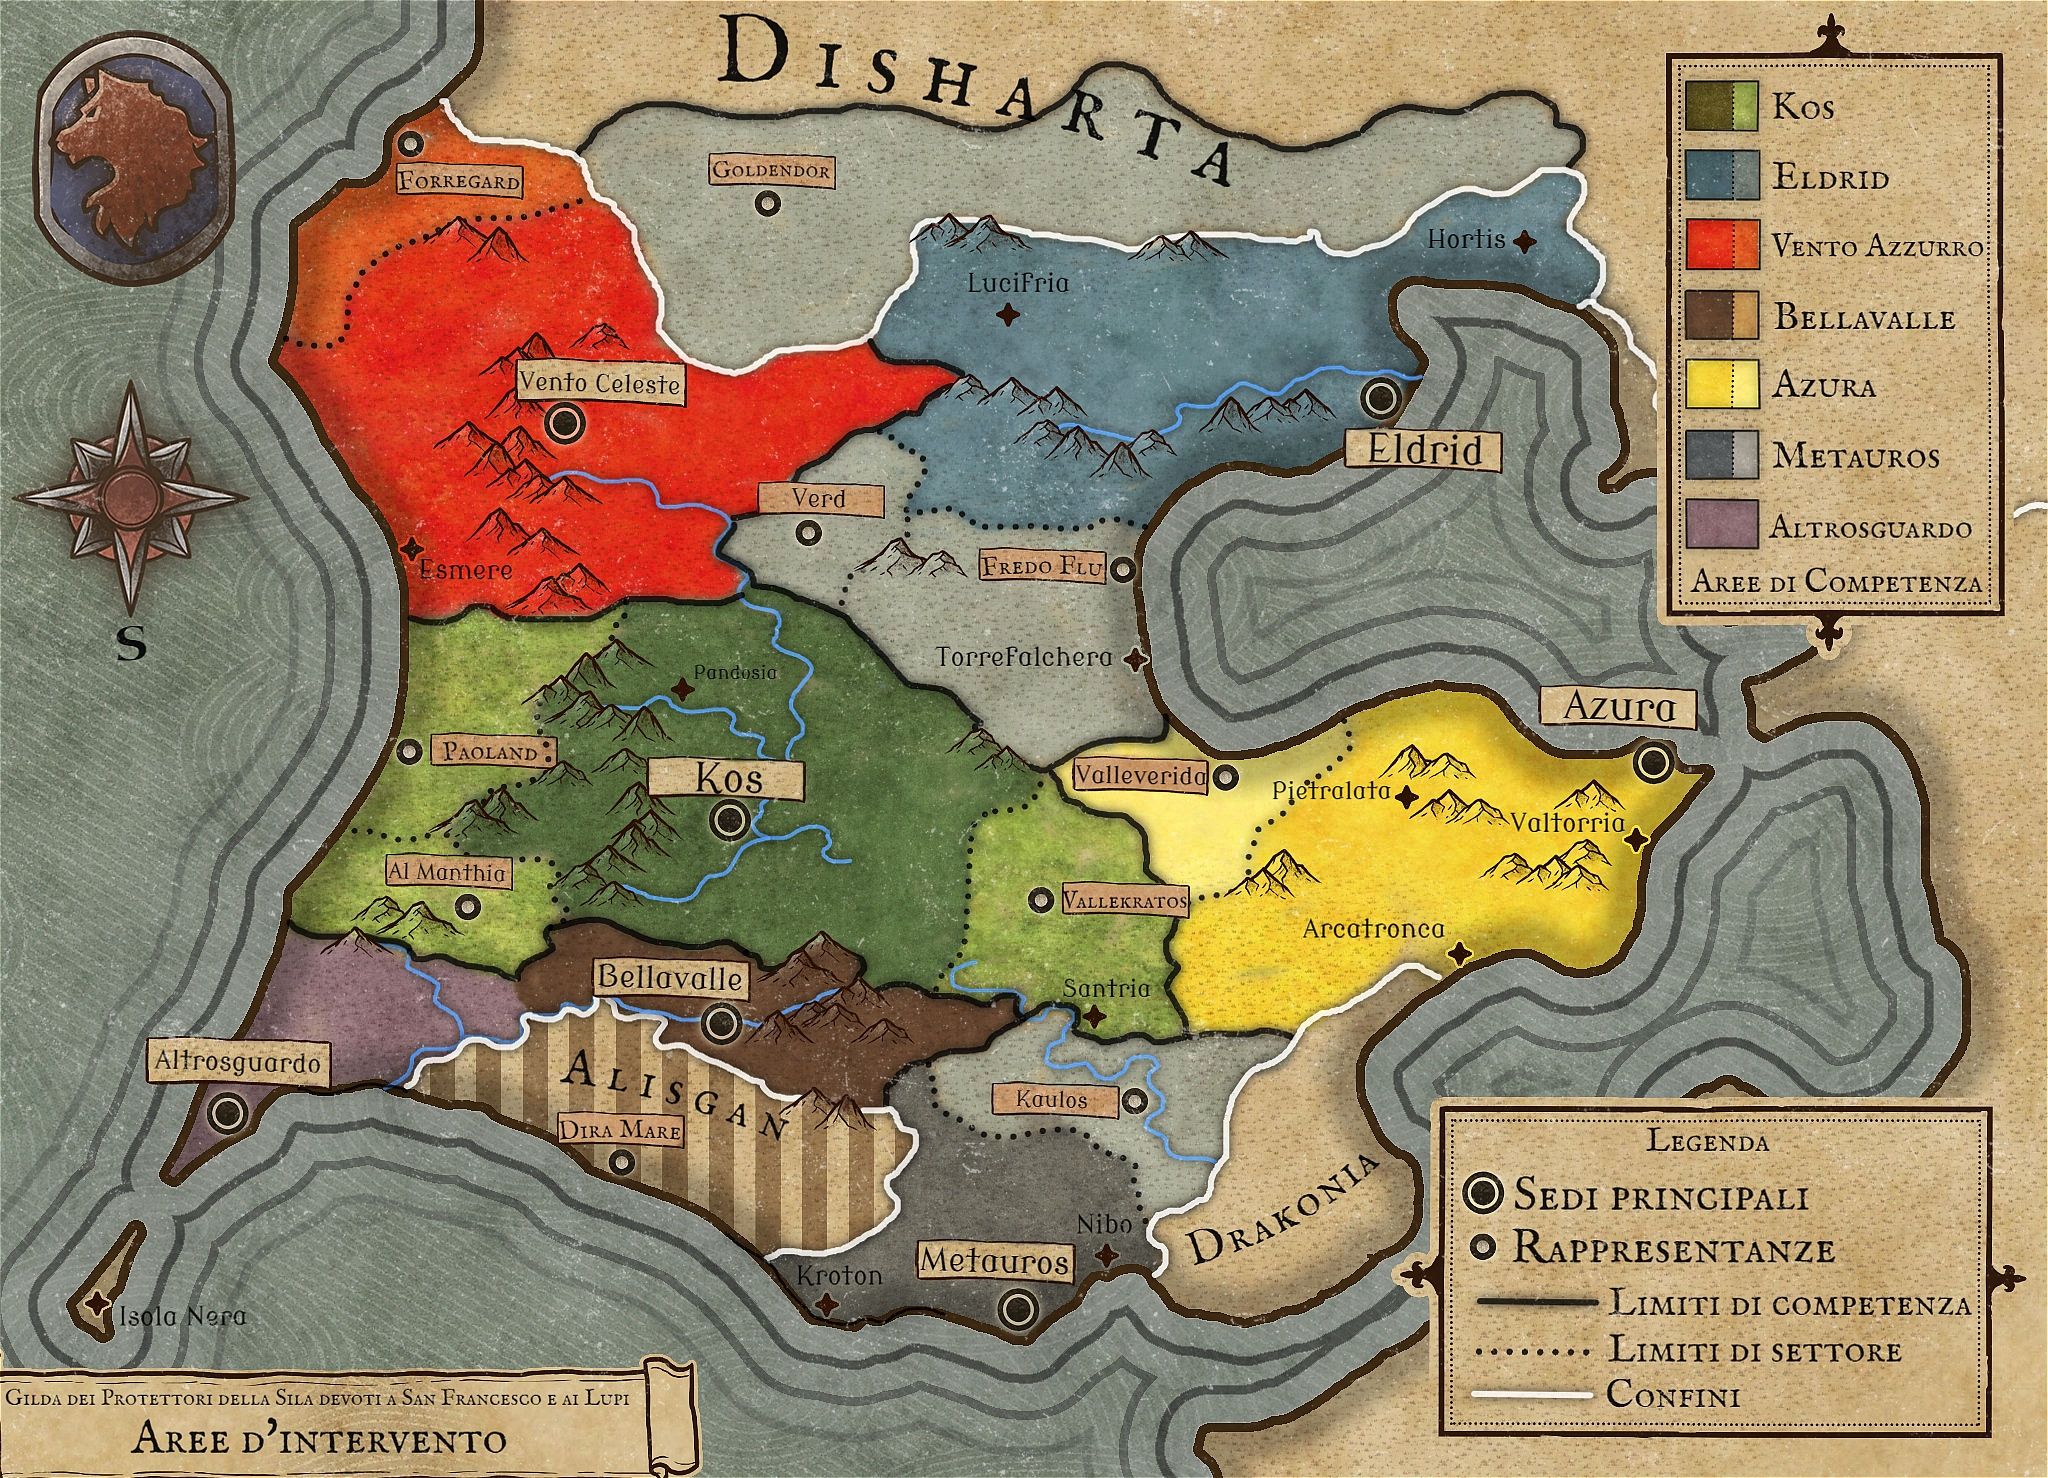
\includegraphics{campo_dazione_gilda_(1).jpg}
\caption{campo d'azione gilda (1).jpg}
\end{figure}

\subsection{6. Struttura gerarchica}\label{struttura-gerarchica}

\begin{center}\rule{0.5\linewidth}{0.5pt}\end{center}

Il \textbf{Consiglio Supremo} è il massimo organo direttivo della Gilda
dei Protettori, e ha autorità su tutte le sedi della gilda sparse per
Valtara. La responsabilità principale del Consiglio è quella di prendere
decisioni strategiche a livello globale e guidare la gilda nella sua
missione di proteggere Valtara da ogni minaccia.

\begin{itemize}
\tightlist
\item
  Il Consiglio, un organismo flessibile, può essere composto da un
  numero variabile di membri (sempre dispari), selezionati in base ai
  meriti, sia internamente che esternamente alla gilda: rinomati uomini
  politici, filantropi, o comunque persone con una comprovata dedizione
  al bene e alla tutela degli indifesi.
\item
  Le riunioni del Consiglio sono pianificate periodicamente, ma la sua
  sede è mobile. La scelta del luogo di incontro dipende da fattori di
  convenienza e urgenza (ad esempio, se si devono affrontare questioni
  relative alla sede di Azura, la riunione si terrà ad Azura). La
  partecipazione dei Comandanti Generali delle diverse sedi alle
  riunioni è altamente consigliata, sebbene non obbligatoria.
\end{itemize}

\subsubsection{\texorpdfstring{6.1 \textbf{Posizioni principali
all'interno di ogni sede della
Gilda}}{6.1 Posizioni principali all'interno di ogni sede della Gilda}}\label{posizioni-principali-allinterno-di-ogni-sede-della-gilda}

\begin{itemize}
\tightlist
\item
  \textbf{Comandante Generale:} Ogni sede della gilda ha un Comandante
  Generale che funge da leader locale. Questi individui sono
  responsabili delle operazioni quotidiane della loro sede, coordinando
  le missioni e supervisionando i membri della gilda assegnati a quella
  sede specifica. Sono nominati dal Consiglio e devono dimostrare
  competenza e leadership.
\item
  \textbf{Ufficiali Superiori:} Sotto il Comandante Generale, ci sono
  gli Ufficiali Superiori. Questi ufficiali sono responsabili di
  specifici settori o divisioni all'interno della sede, come la
  formazione delle reclute, la logistica o la strategia. Collaborano
  direttamente con il Comandante Generale e aiutano a prendere decisioni
  importanti.
\item
  \textbf{Capitani di Squadra:} I Capitani di Squadra sono Protettori
  che si sono particolarmente distinti nella loro carriera per coraggio
  e dedizione alla causa. Sono responsabili del comando e del controllo
  delle unità operative della gilda. Ad una squadra viene assegnato un
  capitano per missioni altamente pericolose o di vitale importanza.
\item
  \textbf{Protettori Esperti:} Questi sono avventurieri esperti che
  costituiscono la forza principale della gilda. Sono responsabili
  dell'esecuzione delle missioni assegnate loro e svolgono un ruolo
  cruciale nella protezione di Valtara.
\item
  \textbf{Reclute:} I nuovi membri che si uniscono alla gilda iniziano
  come reclute. Vengono addestrati e sottoposti a un periodo di prova
  per dimostrare le loro abilità e il loro impegno. Una volta dimostrata
  la loro competenza, possono avanzare a posizioni superiori.
\end{itemize}

\subsubsection{\texorpdfstring{6.2 \textbf{Altre
posizioni}}{6.2 Altre posizioni}}\label{altre-posizioni}

\begin{itemize}
\tightlist
\item
  \textbf{Quartiermastro:} Il Quartiermastro è responsabile della
  gestione delle risorse materiali della gilda, inclusi armamenti,
  equipaggiamento e rifornimenti. Assicura che tutto il personale abbia
  ciò di cui ha bisogno per le operazioni.
\item
  All'interno della gilda ci sono anche posizioni amministrative come
  scribi, responsabili della documentazione delle missioni, o logistici,
  incaricati della gestione delle risorse e dell'approvvigionamento.
\end{itemize}

\href{Untitled\%20Database\%2077b97fb33d1b4871909da1f0d726e8dc.csv}{Untitled
Database}
